\documentclass{standalone}
\usepackage{tikz}
\usepackage{ctex,siunitx,ninecolors}
\setCJKmainfont{Noto Serif CJK SC}
\usepackage{tkz-euclide}
\usepackage{amsmath}
\usepackage{wasysym}
\usetikzlibrary{patterns, calc}
\usetikzlibrary {decorations.pathmorphing, decorations.pathreplacing, decorations.shapes,backgrounds}
\begin{document}
\small
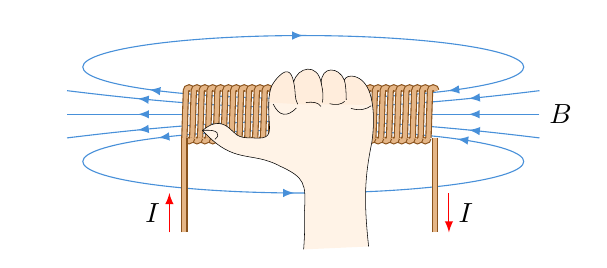
\begin{tikzpicture}[>=latex,scale=1]
  \useasboundingbox(-3.5,-1.6)rectangle(3.5,1.1);
  \foreach \x/\y in {7/0.3,0/0,-7/-0.3}
  {
    \draw[azure6,postaction={decorate},decoration={markings,mark=between positions 0.15 and 0.9 step 0.7 with {\arrow{>}}}](3,\y)to[bend left=\x](-3,\y);
  }
  \draw[azure6,postaction={decorate},decoration={markings,mark=between positions 0.25 and 1.0 step 0.33 with {\arrowreversed{>}}}](0,0.6)ellipse(2.8 and 0.4);
  \draw[azure6,postaction={decorate},decoration={markings,mark=between positions 0.08 and 0.8 step 0.33 with {\arrow{>}}}](0,-0.6)ellipse(2.8 and 0.4);
  \node at (3,0) [right]{$B$};
  \draw[brown4,double=brown8,double distance=1.5pt](-1.51,-0.3)--(-1.49,0.3)arc(180:0:0.04);
  \foreach \x in {-1.4,-1.3,...,1.6}
  {
    \draw[brown4,double=brown8,double distance=1.5pt](\x-0.01,-0.3)--(\x+0.01,0.3)arc(180:0:0.04);
    \draw[brown4,double=brown8,double distance=1.5pt](-\x+0.19,-0.3)arc(0:-180:0.04);
  }
  \draw[brown4,double=brown8,double distance=1.5pt](-1.51,-1.5)--(-1.51,-0.3);
  \draw[brown4,double=brown8,double distance=1.5pt](1.67,-1.5)--(1.67,-0.3);
  \draw[red,->,text=black](-1.7,-1.5)--++(0,0.5)node[midway,left]{$I$};
  \draw[red,->,text=black](1.85,-1.0)--++(0,-0.5)node[midway,right]{$I$};
  \begin{scope}[xshift=3mm,yshift=-4mm]
    \fill[pink!10!orange!10,draw=black,very thin]
    (-0.295,-1.316)..controls(-0.274,-1.024)and(-0.284,-0.928)..(-0.284,-0.821)..controls(-0.267,-0.486)and(-0.276,-0.406)..(-0.587,-0.262)..controls(-0.975,-0.055)and(-1.169,-0.252)..(-1.578, 0.194)..controls(-1.435, 0.323)and(-1.319, 0.296)..(-1.233, 0.218)..controls(-1.155, 0.161)and(-1.160, 0.094)..(-0.938, 0.100)..controls(-0.728, 0.080)and(-0.721, 0.151)..(-0.731, 0.285)..controls(-0.735, 0.371)and(-0.741, 0.464)..(-0.738, 0.552)--(-0.581, 0.677)--(-0.187, 0.719)--( 0.106, 0.694)--( 0.408, 0.628)--( 0.579, 0.519)..controls( 0.598, 0.383)and( 0.596, 0.221)..( 0.571, 0.044)..controls( 0.481,-0.391)and( 0.466,-0.682)..( 0.530,-1.279);
    \fill[pink!10!orange!15,draw=black,very thin]
    (-0.738,0.552)..controls(-0.734,0.664)and(-0.715,0.766)..
(-0.657,0.829)..controls(-0.519,1.002)and(-0.451,0.957)..
(-0.422,0.809)..controls(-0.391,0.668)and(-0.416,0.613)..(-0.371,0.528)
(-0.371,0.528)..controls(-0.416,0.613)and(-0.391,0.668)..
(-0.422,0.809)..controls(-0.371,1.006)and(-0.114,1.055)..
(-0.072,0.795)..controls(-0.073,1.019)and( 0.156,1.005)..
( 0.221,0.834)..controls( 0.250,0.924)and( 0.467,0.914)..
( 0.547,0.665)..controls( 0.561,0.621)and( 0.571,0.572)..( 0.579,0.519);
    \draw[very thin] (-0.682,0.530)..controls(-0.606,0.368)and(-0.501,0.364)..(-0.388,0.479)
    (-0.268,0.548)..controls(-0.171,0.562)and(-0.114,0.551)..(-0.074,0.500)
    (-0.072,0.795)..controls(-0.045,0.675)and(-0.046,0.632)..(-0.056,0.552)
    ( 0.035,0.535)..controls( 0.126,0.512)and( 0.189,0.528)..( 0.225,0.564)
    ( 0.221,0.834)..controls( 0.239,0.785)and( 0.243,0.709)..( 0.246,0.584)
    ( 0.306,0.476)..controls( 0.419,0.438)and( 0.506,0.466)..( 0.562,0.508)
    (-1.578,0.194)..controls(-1.379,0.215)and(-1.345,0.143)..(-1.422,0.081);
  \end{scope}
\end{tikzpicture}
\end{document}